\documentclass[10pt,twocolumn]{article}

\usepackage[margin=0.75in]{geometry}
\usepackage{graphicx}
\usepackage{booktabs}
\usepackage{amsmath}
\usepackage{hyperref}
\graphicspath{{paper_figs/}}

\title{Replacing PyArrow with arrow-rs for Parquet Reads in Ray Data}
\author{Aarrya Saraf}
\date{\today}

\begin{document}

\maketitle

\section{Introduction}
For this document, we restrict ourselves to the Ray Data Parquet Reader in Datasource
v2. All the numbers and testing were done on a 8CPU-32GB node running linux on the
Anyscale workspace.

Consider \href{https://github.com/ray-project/ray/issues/49158}{this github issue} which
highlights a known memory leak (I use the word leak loosely here. Testing, at least in
the modern version of Ray, shows more of a transient peak. There seems to be no memory
retention or constant increase) in pyarrow which, by extension, causes leaks in Ray Data
when reading certain parquet files. Currently, when scheduling read tasks, we do not take
this memory into account. Instead we pass CPU constraints onto core. For such cases, the
scheduler, unaware of this leak, can keep on adding read tasks on the same machine
causing OOMs. This prototype explores whether switching to arrow-rs (the rust equivalent)
can resolve this issue.

\subsection{Background: Parquet}
Parquet files store tables with one schema at the file level. Inside a file, the table is
divided into horizontal slices called row groups and inside each row group, we store the
data in a columnar format (which is stored in data pages). There are some optional
statistics like min, max, bloom filters, and more for each column chunk and for pages.
The page sizes are user controlled but generally 1 MiB in size.

\subsection{PyArrow vs Arrow-rs}
In the current datasource v2 implementation, we use the scan\_batches function for
multiple reasons like schema unification, filter pushdown and prefetching that
iter\_batches does not offer out of the box. This function decodes the entire row-group
in memory so it holds the decoded row group in memory. iter\_batches is slightly better
holding the compressed row group in memory and would be a python only improvement without
external dependencies. However, this isn't free either. This win is seen only for large
row groups but the overhead of iter\_batches actually makes memory worse for a small row
group. Arrow-rs on the other hand has a bounded window. It does not have all the in built
benefits of scan\_batches but those can be wrapped around it. Below we show an evaluation
of all 3 against one another.

\emph{The mechanism, briefly.} PyArrow's decode unit is a whole row group, so a worker's
peak private heap grows with the group the file dictates. arrow-rs sizes each decode
batch by bytes --- from the footer it picks a row count so
$\text{rows}\times\text{bytes/row}\approx\text{budget}$ (a few MiB), dropping each batch
as the next is pulled --- turning the $O(\text{row group})$ term into $O(\text{budget})$:
a working set we set, not one the file dictates.

\section{Experimental Methodology}
\emph{Setup.} We compare three readers on identical fixtures with per-column hash parity,
so any memory gap is a pure decoder effect: the PyArrow scanner (Ray's V2 default,
\texttt{pre\_buffer=True}), PyArrow \texttt{iter\_batches}, and arrow-rs. We swept a wide
matrix, one variable at a time: storage (local vs.\ real S3), row-group size, decode batch
size, schema (ints, floats, strings, and rich types --- Ray tensors and the canonical
\texttt{fixed\_shape\_tensor} extension), file length, file count / concurrency, and
mixed-schema multi-file datasets --- each under scan, \texttt{sum}, and \texttt{filter}
workloads.

\emph{Metric.} Node OOM is driven by resident private memory the scheduler never sees: it
admits tasks on CPU slots and expected output-block size only, not the decode heap. So
the metric of record is worker USS (pages private to a process, excluding shared libraries
and plasma), plotted as USS vs.\ seconds since task start. Across every ablation
(row-group size, batch size, file count, \dots) arrow-rs holds a consistently smaller
slope --- a flat plateau where PyArrow climbs to the whole decoded group --- which is the
finding, not a single peak.

\emph{Decomposing USS.} A read task's private memory is roughly
\begin{equation*}
\text{USS} \;\approx\; S_\text{in} \;+\; W_\text{decode} \;+\; S_\text{out} \;+\; M_\text{uncontrolled},
\end{equation*}
where $S_\text{in}$ is the input bytes read, $W_\text{decode}$ the decode working set,
$S_\text{out}$ the output block(s) handed to plasma, and $M_\text{uncontrolled}$ memory we
do not manage (e.g.\ freed pages the allocator keeps cached). Give both readers the
\emph{same} large input and output, and only $W_\text{decode}$ differs: arrow-rs holds
$\approx$ one page (its byte budget, a few MiB), whereas PyArrow holds the whole row group
--- encoded under \texttt{iter\_batches}, decoded under the \texttt{scan\_batches} default.
That single term is the entire memory story.

\section{Results}
Table~\ref{tab:results} spans the matrix. Memory (peak worker USS) is lower in every case;
wall time is faster on large fixtures and within a few percent on small ones. Node:
8~vCPU / 32~GB Linux, warm cache.

\begin{table}[t]
\centering
\small
\begin{tabular}{@{}lrr@{}}
\toprule
Workload (rows, RGs, schema) & USS saved & Wall $\Delta$ \\
\midrule
4M, 1 RG, int (scan)              & 55\% & -9\% \\
\quad same, \texttt{filter} (9 int cols) & 75\% & $+$15\% \\
\quad same, \texttt{sum}          & 20\% & $+$8\% \\
500k, 5 RG, \texttt{fixed\_shape\_tensor} & 6\%  & $-$0.2\% \\
500k, 5 RG, float                 & 15\% & $+$9\% \\
500k, 5 RG, string / Ray tensor   & 15\% & $+$5\% \\
Big RG on S3                      & 62\% & $\approx$0 \\
Mixed 6-file (1 struct fallback)  & 35\% & $-$45\% \\
\bottomrule
\end{tabular}
\caption{Breadth of the sweep. \emph{USS saved} $= 1 -$ arrow-rs$/$PyArrow peak private
heap. \emph{Wall $\Delta$}: $+$ slower, $-$ faster. Rich types decode byte-identically;
memory wins everywhere (6--75\%).}
\label{tab:results}
\end{table}

\emph{Row-group size is the lever.} At 4M rows in one row group arrow-rs uses 55\% less
peak USS and is faster, and the gap grows with row-group size --- exactly where PyArrow
must materialize one large indivisible unit. When a file already has many small groups,
Ray's read pool splits it across workers so no worker holds a big group, and the two
readers converge to parity: the correct ``not worse'' outcome.

\emph{Rich types are not a barrier.} Extension and tensor columns
(\texttt{fixed\_shape\_tensor}, Ray's tensor types), strings, and floats all decode
byte-identically and still cut memory 6--15\%. On the small 500k-row fixtures arrow-rs is
a few percent slower (5--9\% --- fixed per-call overhead that a small decode can't
amortize), always paired with the memory win.

\emph{Workloads and S3.} A \texttt{filter} (4M rows, 9 int cols) uses 75\% less memory for
$+$15\% time, and a \texttt{sum} 20\% less for $+$8\% --- both decode fully today but never
accumulate the group. The target OOM case, a lone big row group as one S3 object, is 62\%
less memory at speed parity: arrow-rs's fetch window caps compressed bytes in flight while
PyArrow pulls the whole object. A
heterogeneous 6-file dataset (one member falling back to PyArrow) still ran 1.8$\times$
faster at 35\% less memory.

\section{Limitations}
The main real cost is Ray Data owning a cross-platform Rust build in CI. On small fixtures
the fixed per-call overhead makes arrow-rs a few percent slower (it is faster once the
decode is large or output is materialized). We prune whole row groups by footer statistics
at parity with PyArrow, but still decode surviving rows before filtering them. And the
clearest win is the ``one big row group'' layout --- worth confirming how often real
customer files hit it.

\section{Future Work}
Beyond the row-group pruning both readers do today, Parquet often carries finer statistics
we do not yet exploit: a page index (per-page min/max plus byte offsets) and, for
equality/\texttt{IN} predicates, bloom filters. When present, these let a reader skip
individual pages and seek directly to the survivors. arrow-rs is well-suited to this ---
it already loads the page index and skips pages via \texttt{RowSelection} for its
range-split path, and parquet-rs supports bloom-filter reads --- so the same machinery can
be driven by a pushed-down filter. Combined with late materialization (decode only the
predicate column, evaluate the filter, then decode the wide columns for surviving rows
only), this turns today's ``decode everything, keep a few'' into ``touch a few pages,
decode a few rows.'' It also composes with Ray's planned page-index chunker, where the
reader must consume sub-row-group page ranges --- something arrow-rs's \texttt{RowSelection}
already does.

\section{Conclusion}
PyArrow decodes a whole row group into a worker's private heap --- memory the scheduler
never accounts for --- so on large row groups it keeps admitting read tasks until the node
OOM-kills. arrow-rs bounds the decode by bytes, making that working set a knob we set
rather than a property of the file. Across our sweep --- storage (local and S3), row-group
and batch sizes, rich types (including tensors and extensions), file counts, mixed schemas,
and scan/filter/sum workloads --- peak worker USS is 6--75\% lower, at parity only when the
file already has many small groups that Ray's pool spreads across workers (the correct
``not worse'' outcome). Speed is faster on large or materialized workloads and within a few
percent on small fixtures, where fixed per-call overhead dominates. The net is a large,
consistent memory win at little-to-no speed cost --- which is what removing the \#49158
OOMs requires.

\appendix
\section{Supplementary figures}
The figures below are from runs on \textbf{macOS}, not the Linux workspace used for the
tables in \S4, so the absolute numbers differ slightly --- the shapes and ratios are the
point. Each plot is worker USS (MB) during the read task vs.\ seconds since task start:
red $=$ PyArrow V2 scanner, orange $=$ PyArrow \texttt{iter\_batches}, blue $=$ arrow-rs.
The table embedded in each figure repeats wall time and peak USS with deltas vs.\ the
scanner.

\begin{figure*}[t]
\centering
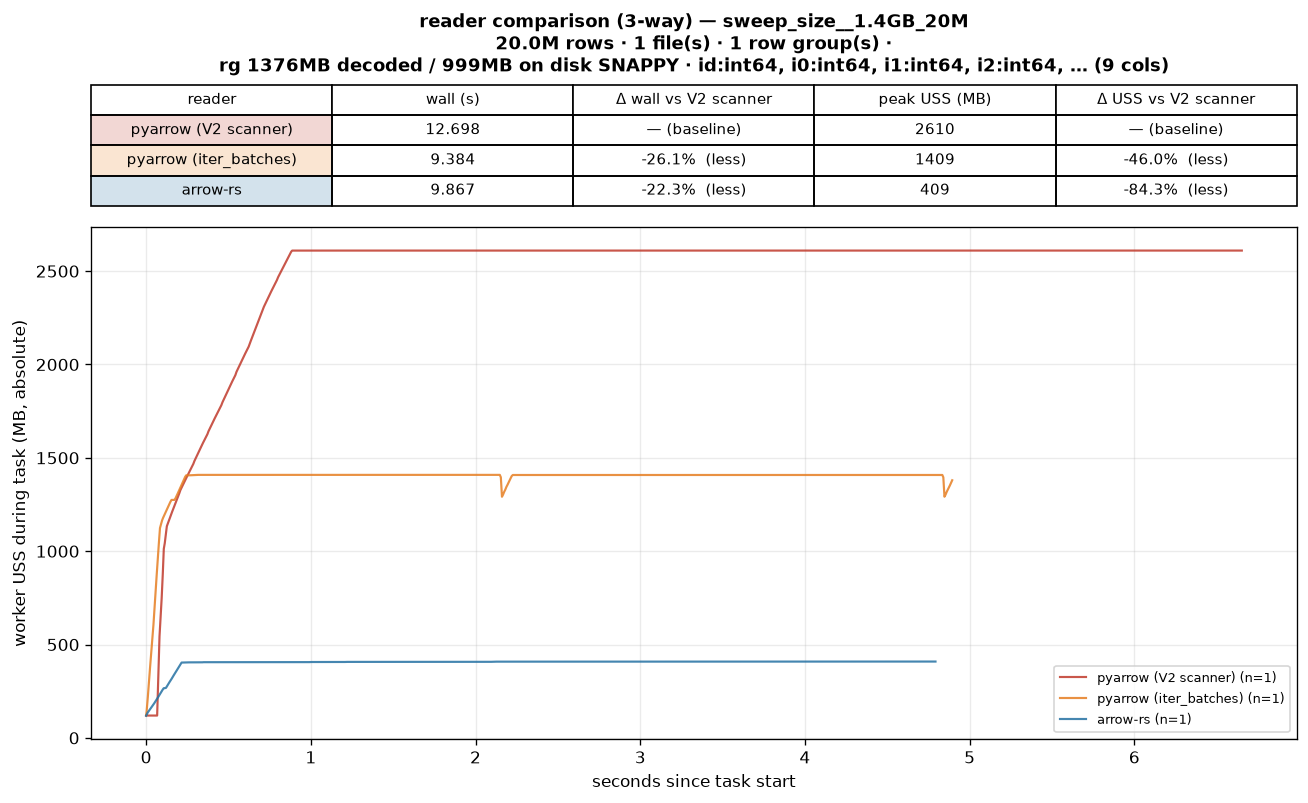
\includegraphics[width=\textwidth]{sweep_1_4gb.png}
\caption{\emph{One lone big row group --- the target case.} 20M rows, 1 file, 1 row group
(1376 MB decoded / 999 MB on-disk snappy), 9 int columns. arrow-rs holds a flat
\textasciitilde410 MB while the PyArrow scanner climbs to \textasciitilde2.6 GB
($-$84\% USS) and \texttt{iter\_batches} plateaus at \textasciitilde1.4 GB.}
\label{fig:sweep}
\end{figure*}

\begin{figure*}[t]
\centering
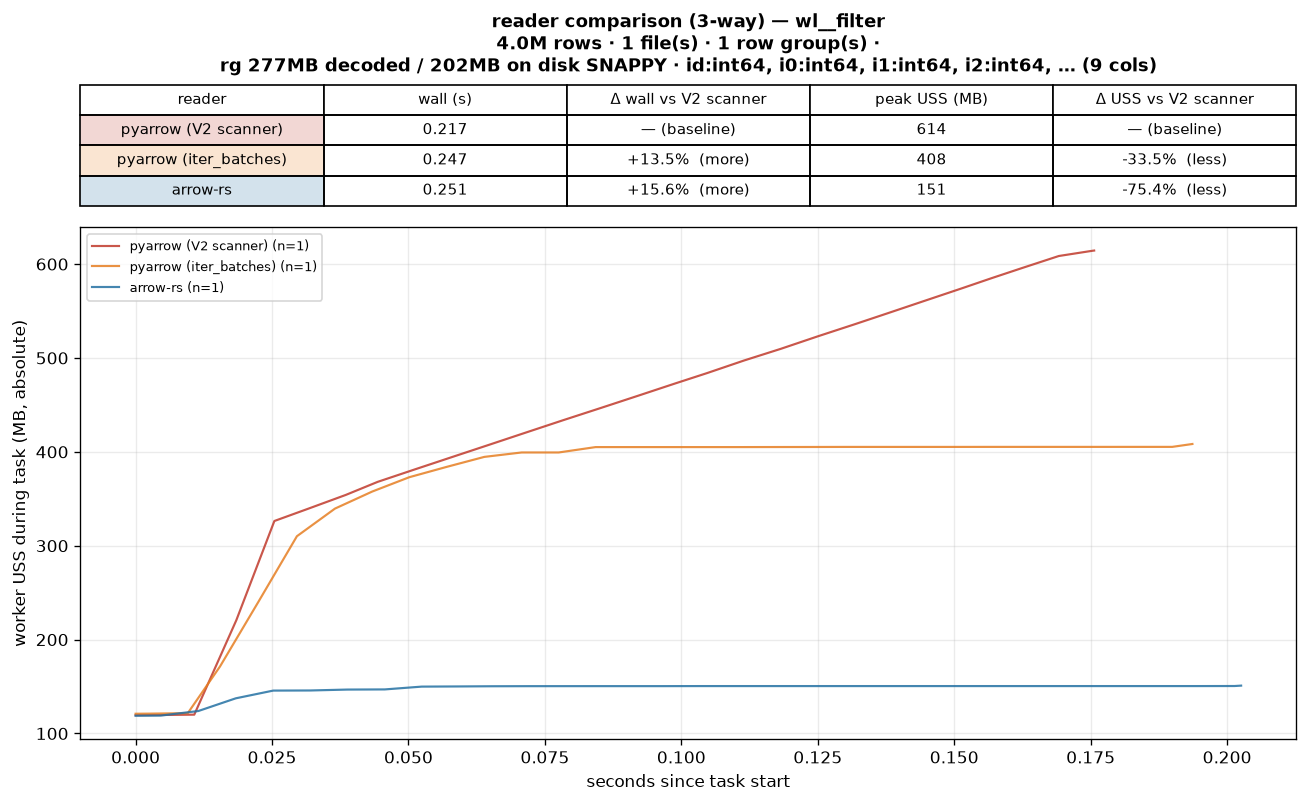
\includegraphics[width=\textwidth]{filter.png}
\caption{\emph{Filter workload.} 4M rows, 1 file, 1 row group (277 MB decoded / 202 MB
on-disk snappy), 9 int columns. All rows are decoded and then filtered; arrow-rs's decode
transient never accumulates, so its peak USS stays far below PyArrow's.}
\label{fig:filter}
\end{figure*}

\begin{figure*}[t]
\centering
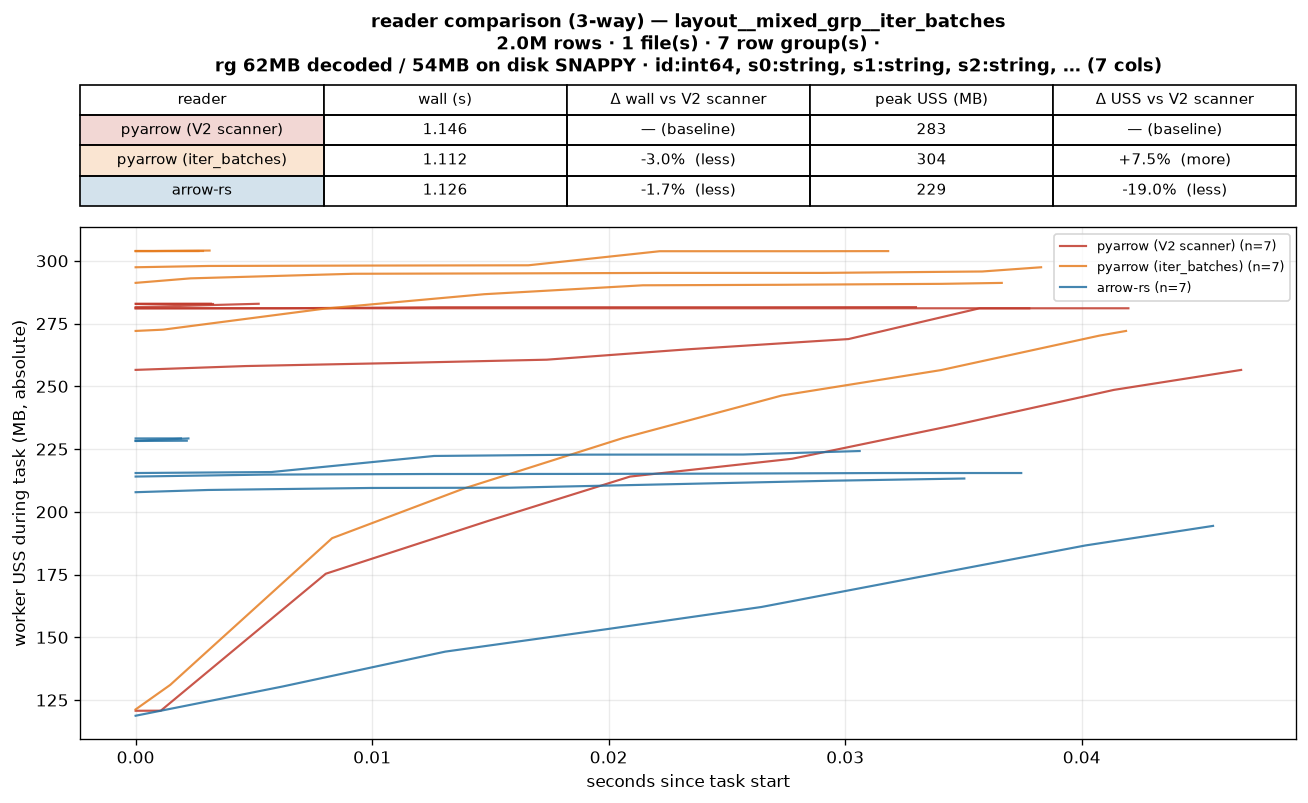
\includegraphics[width=\textwidth]{mixed_grp.png}
\caption{\emph{Mixed row-group sizes.} 2M rows in 7 row groups
(\textasciitilde62 MB decoded / 54 MB on-disk snappy per group), schema $=$ int \texttt{id}
$+$ 6 string columns so per-group size varies; \texttt{iter\_batches} consume. The
per-group fan-out keeps every reader bounded, and arrow-rs stays at or below PyArrow.}
\label{fig:mixed}
\end{figure*}

\end{document}
